\documentclass[border=10pt]{standalone}
\usepackage{tikz}
\usetikzlibrary{arrows.meta, positioning, calc, fit, backgrounds, decorations.pathreplacing, shapes.geometric}

\begin{document}
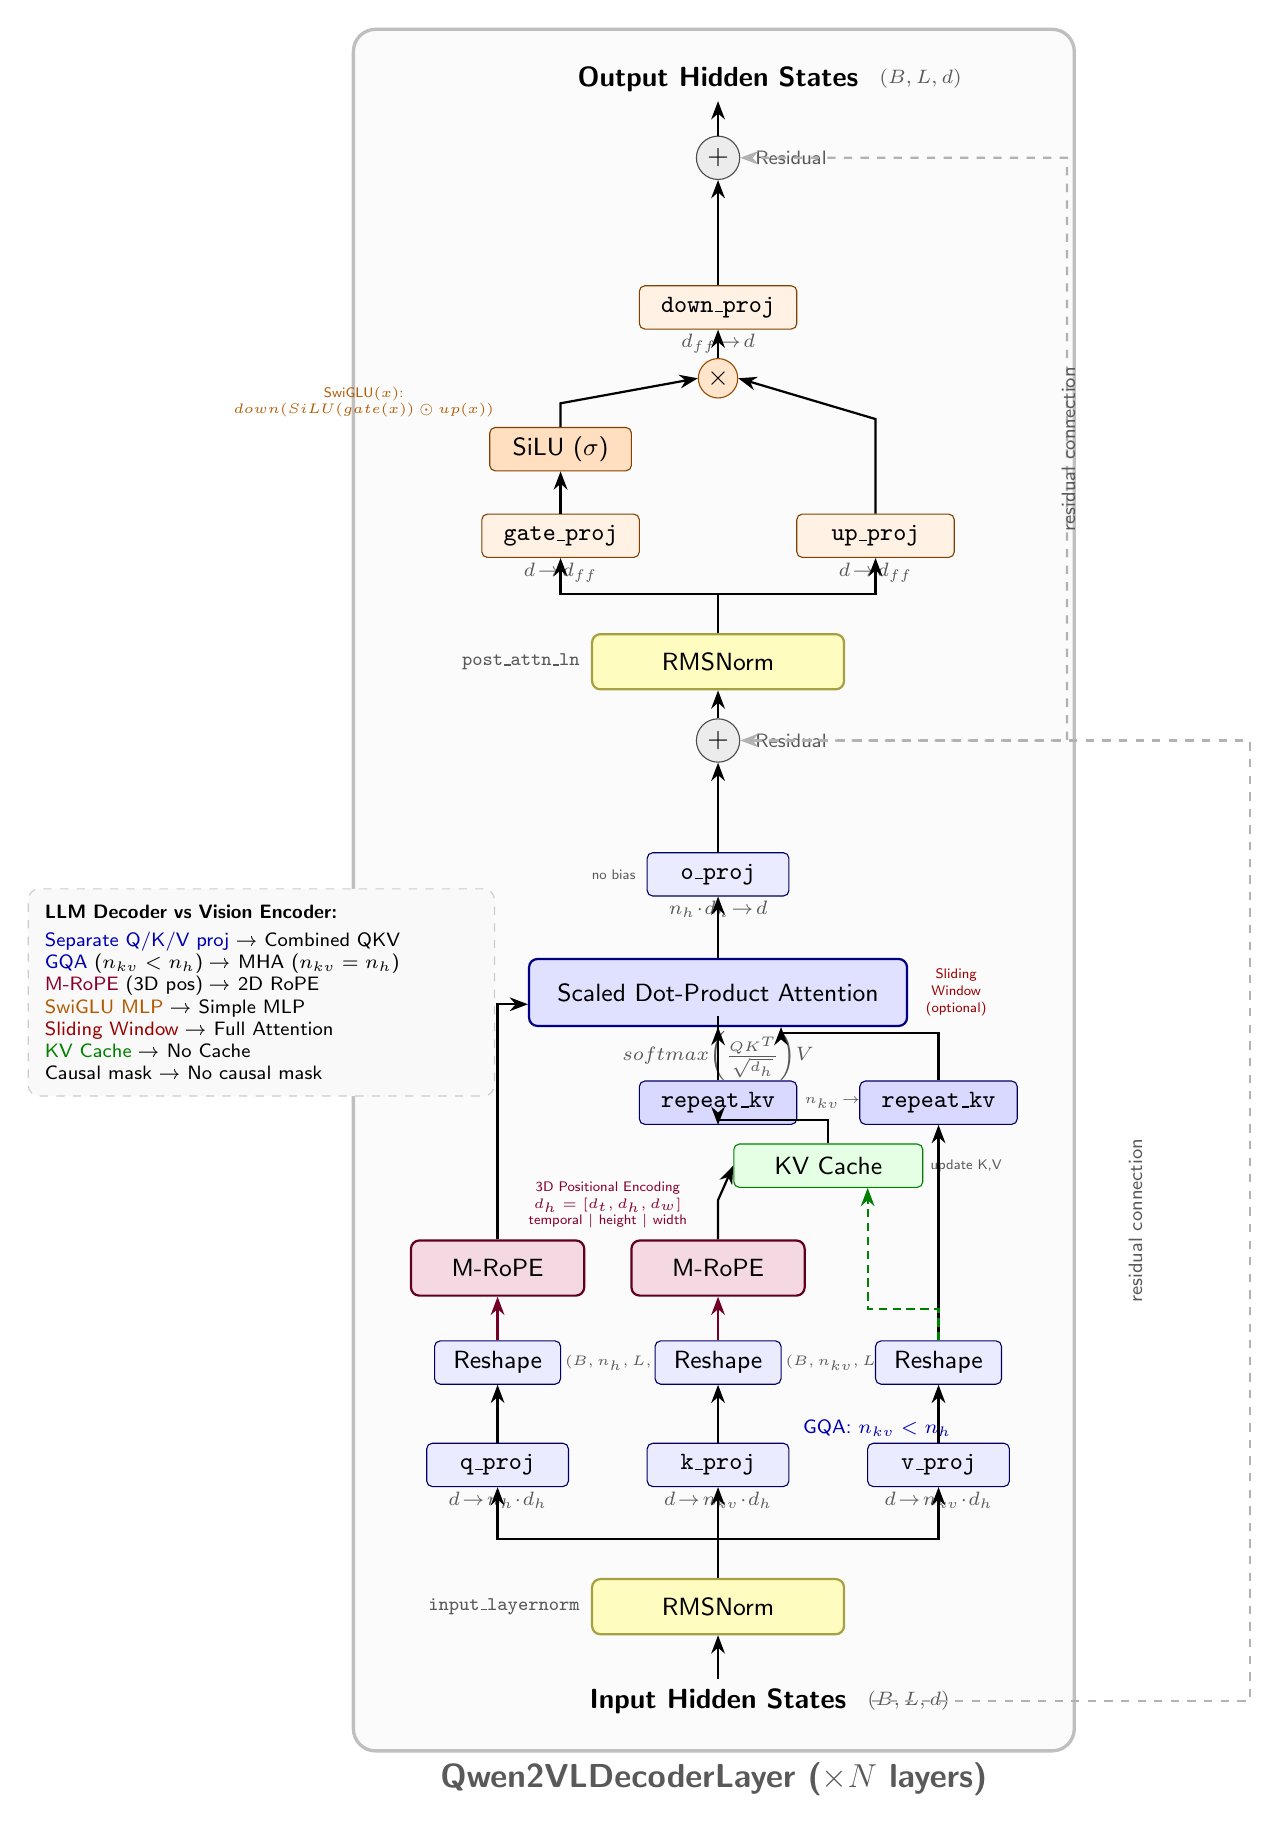
\begin{tikzpicture}[
    % Base styles
    node distance=0.6cm,
    >=Stealth,
    font=\sffamily\small,
    % Box styles
    mainbox/.style={draw, rounded corners=3pt, minimum width=3.2cm, minimum height=0.7cm, align=center, thick},
    normbox/.style={mainbox, fill=yellow!25, draw=yellow!60!black},
    attnbox/.style={mainbox, fill=blue!12, draw=blue!50!black},
    mlpbox/.style={mainbox, fill=orange!15, draw=orange!60!black},
    ropebox/.style={mainbox, fill=purple!15, draw=purple!50!black, minimum width=2.2cm},
    cachebox/.style={draw, rounded corners=2pt, fill=green!10, draw=green!50!black, minimum width=1.6cm, minimum height=0.55cm, align=center},
    addbox/.style={draw, circle, fill=gray!15, draw=gray!60!black, minimum size=0.55cm, inner sep=0pt, font=\sffamily\bfseries},
    projbox/.style={draw, rounded corners=2pt, fill=blue!8, draw=blue!40!black, minimum width=1.8cm, minimum height=0.55cm, align=center},
    projboxS/.style={draw, rounded corners=2pt, fill=blue!8, draw=blue!40!black, minimum width=1.4cm, minimum height=0.55cm, align=center},
    gluebox/.style={draw, rounded corners=2pt, fill=orange!10, draw=orange!50!black, minimum width=1.6cm, minimum height=0.55cm, align=center},
    mulbox/.style={draw, circle, fill=orange!20, draw=orange!60!black, minimum size=0.5cm, inner sep=0pt, font=\sffamily\bfseries},
    dimlab/.style={font=\sffamily\scriptsize\color{gray!70!black}, inner sep=1pt},
    contrastbox/.style={draw, rounded corners=4pt, fill=gray!5, draw=gray!40, dashed, inner sep=6pt, align=left, font=\sffamily\scriptsize},
    groupbox/.style={draw, rounded corners=6pt, thick, inner sep=8pt},
    arrow/.style={->, thick, >=Stealth},
    grayarrow/.style={->, thick, >=Stealth, gray!60, dashed},
]

% ============================================================
% MAIN FLOW (vertical, bottom to top)
% ============================================================

% Input
\node (input) at (0, 0) [font=\sffamily\bfseries] {Input Hidden States};
\node[dimlab, right=0.1cm of input] {$(B, L, d)$};

% Input LayerNorm
\node (ln1) at (0, 1.2) [normbox] {RMSNorm};
\node[dimlab, left=0.1cm of ln1] {\texttt{input\_layernorm}};

% ============================================================
% ATTENTION BLOCK (expanded)
% ============================================================

% Q, K, V projections - separate
\node (qproj) at (-2.8, 3.0) [projbox] {\texttt{q\_proj}};
\node[dimlab, below=0.02cm of qproj] {$d \!\to\! n_h \!\cdot\! d_h$};
\node (kproj) at (0, 3.0) [projbox] {\texttt{k\_proj}};
\node[dimlab, below=0.02cm of kproj] {$d \!\to\! n_{kv} \!\cdot\! d_h$};
\node (vproj) at (2.8, 3.0) [projbox] {\texttt{v\_proj}};
\node[dimlab, below=0.02cm of vproj] {$d \!\to\! n_{kv} \!\cdot\! d_h$};

% GQA annotation
\node[font=\sffamily\scriptsize\color{blue!70!black}, above right=-0.05cm and 0.05cm of kproj] {GQA: $n_{kv} < n_h$};

% Reshape + transpose
\node (qresh) at (-2.8, 4.3) [projboxS, minimum width=1.6cm] {Reshape};
\node[dimlab, right=0.01cm of qresh] {\tiny$(B,n_h,L,d_h)$};
\node (kresh) at (0, 4.3) [projboxS, minimum width=1.6cm] {Reshape};
\node[dimlab, right=0.01cm of kresh] {\tiny$(B,n_{kv},L,d_h)$};
\node (vresh) at (2.8, 4.3) [projboxS, minimum width=1.6cm] {Reshape};

% M-RoPE on Q and K
\node (mrope_q) at (-2.8, 5.5) [ropebox] {M-RoPE};
\node (mrope_k) at (0, 5.5) [ropebox] {M-RoPE};

% M-RoPE detail annotation
\node[font=\sffamily\tiny\color{purple!70!black}, align=center] at (-1.4, 6.3)
    {3D Positional Encoding\\$d_h = [d_t, d_h, d_w]$\\temporal $|$ height $|$ width};

% KV Cache
\node (kvcache) at (1.4, 6.8) [cachebox, minimum width=2.4cm] {KV Cache};
\node[dimlab, right=0.05cm of kvcache] {\tiny update K,V};

% repeat_kv for GQA
\node (repeatk) at (0, 7.6) [projboxS, fill=blue!15, minimum width=2.0cm] {\texttt{repeat\_kv}};
\node[dimlab, right=0.05cm of repeatk] {\tiny$n_{kv} \!\to\! n_h$};
\node (repeatv) at (2.8, 7.6) [projboxS, fill=blue!15, minimum width=2.0cm] {\texttt{repeat\_kv}};

% Scaled Dot-Product Attention
\node (sdpa) at (0, 9.0) [attnbox, minimum width=4.8cm, minimum height=0.85cm]
    {Scaled Dot-Product Attention};
\node[dimlab, below=0.01cm of sdpa] {$\text{softmax}\!\left(\frac{QK^T}{\sqrt{d_h}}\right)\!V$};

% Sliding window annotation
\node[font=\sffamily\tiny\color{red!60!black}, align=center, right=0.1cm of sdpa]
    {Sliding\\Window\\(optional)};

% O projection
\node (oproj) at (0, 10.5) [projbox] {\texttt{o\_proj}};
\node[dimlab, below=0.02cm of oproj] {$n_h \!\cdot\! d_h \!\to\! d$};
\node[dimlab, left=0.1cm of oproj] {\tiny no bias};

% Attention group box
\begin{scope}[on background layer]
\node[groupbox, fill=blue!4, draw=blue!30,
      fit=(qproj)(vproj)(mrope_q)(sdpa)(oproj)(repeatv)(kvcache),
      label={[font=\sffamily\bfseries\small, text=blue!60!black]above:Qwen2VLAttention (GQA + M-RoPE)}] (attngroup) {};
\end{scope}

% Residual Add 1
\node (add1) at (0, 12.2) [addbox] {$+$};
\node[dimlab, right=0.15cm of add1] {Residual};

% Post-attention LayerNorm
\node (ln2) at (0, 13.2) [normbox] {RMSNorm};
\node[dimlab, left=0.1cm of ln2] {\texttt{post\_attn\_ln}};

% ============================================================
% SwiGLU MLP BLOCK (expanded)
% ============================================================

% gate and up projections (parallel)
\node (gate) at (-2.0, 14.8) [gluebox, minimum width=2.0cm] {\texttt{gate\_proj}};
\node[dimlab, below=0.02cm of gate] {$d \!\to\! d_{ff}$};
\node (up) at (2.0, 14.8) [gluebox, minimum width=2.0cm] {\texttt{up\_proj}};
\node[dimlab, below=0.02cm of up] {$d \!\to\! d_{ff}$};

% SiLU activation
\node (silu) at (-2.0, 15.9) [gluebox, fill=orange!25, minimum width=1.8cm] {SiLU ($\sigma$)};

% Element-wise multiply
\node (mul) at (0, 16.8) [mulbox] {$\times$};

% Down projection
\node (down) at (0, 17.7) [gluebox, minimum width=2.0cm] {\texttt{down\_proj}};
\node[dimlab, below=0.02cm of down] {$d_{ff} \!\to\! d$};

% MLP group box
\begin{scope}[on background layer]
\node[groupbox, fill=orange!4, draw=orange!30,
      fit=(gate)(up)(silu)(mul)(down),
      label={[font=\sffamily\bfseries\small, text=orange!60!black]above:Qwen2MLP (SwiGLU)}] (mlpgroup) {};
\end{scope}

% Residual Add 2
\node (add2) at (0, 19.6) [addbox] {$+$};
\node[dimlab, right=0.15cm of add2] {Residual};

% Output
\node (output) at (0, 20.6) [font=\sffamily\bfseries] {Output Hidden States};
\node[dimlab, right=0.1cm of output] {$(B, L, d)$};

% ============================================================
% ARROWS - Main flow
% ============================================================

% Input -> LN1
\draw[arrow] (input) -- (ln1);

% LN1 -> Q, K, V (fan out)
\draw[arrow] (ln1.north) -- ++(0, 0.5) -| (qproj.south);
\draw[arrow] (ln1.north) -- ++(0, 0.5) -- (kproj.south);
\draw[arrow] (ln1.north) -- ++(0, 0.5) -| (vproj.south);

% Q,K,V -> reshape
\draw[arrow] (qproj) -- (qresh);
\draw[arrow] (kproj) -- (kresh);
\draw[arrow] (vproj) -- (vresh);

% Reshape -> M-RoPE (Q, K only)
\draw[arrow, purple!60!black] (qresh) -- (mrope_q);
\draw[arrow, purple!60!black] (kresh) -- (mrope_k);

% V bypass M-RoPE -> goes to repeat_kv
\draw[arrow] (vresh.north) -- ++(0, 0.4) -- ++(0, 0.8) -- (repeatv.south);

% M-RoPE Q -> SDPA
\draw[arrow] (mrope_q.north) -- ++(0, 0.5) -- ++(-0.0, 0) |- ([yshift=-0.15cm]sdpa.west);

% M-RoPE K -> KV Cache -> repeat_kv
\draw[arrow] (mrope_k.north) -- ++(0, 0.5) -- (kvcache.west);
\draw[arrow] (kvcache.north) -- ++(0, 0.3) -| (repeatk.south);

% V -> KV Cache (also)
\draw[arrow, green!50!black, densely dashed] (vresh.north) -- ++(0, 0.4) -| ([xshift=0.5cm]kvcache.south);

% repeat_kv -> SDPA
\draw[arrow] (repeatk.north) -- ++(0, 0.4) -- (sdpa.south -| repeatk.north) -- ([yshift=0.0cm]sdpa.south);
\draw[arrow] (repeatv.north) -- ++(0, 0.4) -- ++(0, 0.2) -| ([xshift=0.8cm]sdpa.south);

% SDPA -> O proj
\draw[arrow] (sdpa) -- (oproj);

% O proj -> Add1
\draw[arrow] (oproj) -- (add1);

% Residual 1: Input -> Add1 (bypass)
\draw[grayarrow] ([xshift=0.2cm]input.east) -- ++(4.8, 0) -- ++(0, 12.2) -- (add1.east);
\node[dimlab, rotate=90] at (5.3, 6.1) {residual connection};

% Add1 -> LN2
\draw[arrow] (add1) -- (ln2);

% LN2 -> gate, up (fan out)
\draw[arrow] (ln2.north) -- ++(0, 0.5) -| (gate.south);
\draw[arrow] (ln2.north) -- ++(0, 0.5) -| (up.south);

% Gate -> SiLU
\draw[arrow] (gate) -- (silu);

% Up -> mul
\draw[arrow] (up.north) -- ++(0, 1.2) -- (mul.east);

% SiLU -> mul
\draw[arrow] (silu.north) -- ++(0, 0.3) -- (mul.west);

% mul -> down
\draw[arrow] (mul) -- (down);

% down -> add2
\draw[arrow] (down.north) -- ++(0, 0.5) -- (add2.south);

% Residual 2: Add1 -> Add2 (bypass)
\draw[grayarrow] ([xshift=0.15cm]add1.east) -- ++(4.0, 0) -- ++(0, 7.4) -- (add2.east);
\node[dimlab, rotate=90] at (4.45, 15.9) {residual connection};

% Add2 -> Output
\draw[arrow] (add2) -- (output);

% ============================================================
% SwiGLU formula annotation
% ============================================================
\node[font=\sffamily\tiny\color{orange!70!black}, align=center] at (-4.5, 16.5)
    {SwiGLU$(x)$:\\$\text{down}(\text{SiLU}(\text{gate}(x)) \odot \text{up}(x))$};

% ============================================================
% CONTRAST with Vision Block
% ============================================================
\node[contrastbox, text width=5.5cm] at (-5.8, 9.0) {
    \textbf{LLM Decoder vs Vision Encoder:}\\[2pt]
    \textcolor{blue!70!black}{Separate Q/K/V proj} \textrightarrow{} Combined QKV\\
    \textcolor{blue!70!black}{GQA} ($n_{kv} < n_h$) \textrightarrow{} MHA ($n_{kv} = n_h$)\\
    \textcolor{purple!70!black}{M-RoPE} (3D pos) \textrightarrow{} 2D RoPE\\
    \textcolor{orange!70!black}{SwiGLU MLP} \textrightarrow{} Simple MLP\\
    \textcolor{red!60!black}{Sliding Window} \textrightarrow{} Full Attention\\
    \textcolor{green!50!black}{KV Cache} \textrightarrow{} No Cache\\
    Causal mask \textrightarrow{} No causal mask
};

% ============================================================
% Outer decoder layer label
% ============================================================
\begin{scope}[on background layer]
\node[draw, rounded corners=8pt, very thick, draw=gray!50, fill=gray!3,
      fit=(input)(output)(attngroup)(mlpgroup),
      inner xsep=12pt, inner ysep=10pt,
      label={[font=\sffamily\bfseries\large, text=gray!70!black]below:Qwen2VLDecoderLayer ($\times N$ layers)}] {};
\end{scope}

\end{tikzpicture}
\end{document}
